\textbf{Programs as Data} 
In order to ease into macros, it's important to understand the basic concepts of why macros exist and what functions they serve.
Macros essentially function as a way of representing \textit{programs as data}.
Up until now, all of our programs have taken data -- ints, strings, floats, and more -- and manipulated such data for the purposes of calculations, object manipulation, data structure creation, and more!

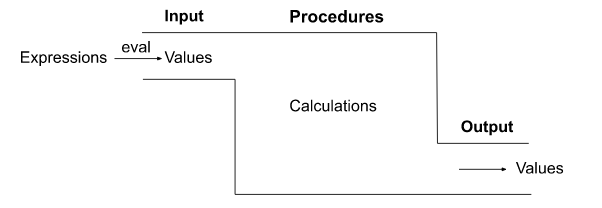
\includegraphics{macro_black_box.png}
\caption{Credit: Rachel de Jaen and Kevin Li, CS 61A Fall 22 Macros Guide}

The purpose of macros is to take full, unevaluated expressions, and treat them as "variables" for which we can take their expression form and evaluate them within the "black box" of the macro, eventually outputting an expression that can be interpreted regularly.
This process requires us to store expressions themselves, not their outputs -- be it primitive, a function, or more -- as data for which the macro can manipulate.

\newpage
\textbf{Macros Overview} Whereas normal Scheme evaluation entails evaluating the operator, then evaluating the operands, before finally applying the operator on operands, macros evaluation involves three steps:

\begin{enumerate}[1.]
\item Evaluate the operator
\item Apply the macro procedure (read: body) to the \textit{unevaluated} operands
\item Evaluate the expression produced by the macro procedure (read: body) in the same frame it was called in and return the result.
\end{enumerate}

This may look overwhelming at first, but just note that the key difference between macro procedures and regular procedures is that the expressions taken as input aren't evaluated before running the body of the macro procedure.
Because the body is evaluated without evaluating the operands at first, macros allow us to implement new special forms, control the order of evaluation, and more. 

Below is a simple example of a macro. Note that even though we pass in \texttt{(print 'hello)} as an operands, we don't evaluate the expression and print right away. Instead we first evaluate the body of the macro procedure, and afterwards we evaluate the expression produced by the macro. 
\vspace{1cm}
\begin{lstlisting}
(define-macro (twice expr)
    (list 'begin expr expr)
)

scm> (twice (print 'hello))
hello
hello
\end{lstlisting}

When \texttt{twice} is called, it will first generate a Scheme list that looks like \texttt{(list 'begin '(print 'hello) '(print 'hello))} (the input is automatically quoted rather than evaluated).

The interpreter will then automaticaly call \texttt{eval} on this list of literals to treat it as if you had just typed it into the interpreter directly. 

\newpage
\textbf{Quoting, Quasiquoting, Unquoting} All Scheme expressions are lists except for atomic expressions like numbers and symbols; so call expressions and special forms are lists too; Example: (+ 1 2)

The \texttt{(quote expression)} special form, also denoted by a \textbf{\'}, simply returns \texttt{expression} - it does not evaluate it. 
This means we can write a Scheme expression and have the expression remain as an expression; if an expression is a call expression or special form, this means the expression will remain a list. 
Quotes return everything to the right of them unevaluated. Here are some brief examples:

\begin{lstlisting}
scm> '(+ 3 4)
(+ 3 4)
\end{lstlisting}
\begin{lstlisting}
scm> (+ 3 4)'
7
\end{lstlisting}
\begin{lstlisting}
scm> (* 3 3)'(* 3 3)
9
(* 3 3)
\end{lstlisting}
Quote wisely! If you throw a quote in the middle of an expression that's to be evaluated a specific way, say (+ 3 '4), you'll run into an operand error!

The \texttt{(quasiquote expression)} special form, \textbf{\`}, has the same effect as \texttt{quote}, except that any expression within \texttt{expression} can be unquoted by preceding it with \texttt{,} or the \texttt{unquote} special form; any unquoted expression is evaluated, whereas everything else within \texttt{expression} is not, as normal. 
As a way of equating quasiquote to Python, quasiquote acts as an f-string of sorts. Take the following Python expression, for example:

\begin{lstlisting}
def cool_string(tens_digit, ones_digit, letter):
    return f"My favorite course at Berkeley is {tens_digit}{ones_digit}{letter}"

>>> cool_string(6, 1, "a")
'My favorite course at Berkeley is 61a"
\end{lstlisting}

Its quasiquoted equivalent in Scheme would be:

\begin{lstlisting}
(define tens_digit 6)
(define ones_digit 1)
(define letter "a")

scm> `(My favorite course at Berkeley is ,tens_digit ,ones_digit ,letter)
(my favorite course at berkeley is 6 1 a)
\end{lstlisting}

Anything denoted with a , preceding it acts as variable in brackets as in the f-string.


Quasiquote and unquote are often used in the body of macro procedures to selectively evaluate certain parts. 

\texttt{(eval expression)} is a procedure that simply evaluates its argument. Note that since \texttt{eval} is a procedure, \texttt{expression} is evaluated first before applying \texttt{eval}.

To build off of the \texttt{twice} example introduced earlier, it is possible to replace all \texttt{list} or \texttt{cons} operations with an expression involving quotes, quasiquotes, and unquotes to produce an identical result:

\begin{lstlisting}
(define-macro (twice expr)
    `(begin ,expr ,expr)
)

scm> (twice (print 'hello))
hello
hello
\end{lstlisting}
